\section{Problem Description}

\begin{frame}
	\frametitle{Physics}
	A set of $N$ massive bodies (``particles''), $m_i$, with positions $\mvec{r}_i=(x_i,y_i)$, $i=0,\ldots,N-1$ are subjected to a symmetric gravitational force, $i\neq j$
	\begin{align*}
		\mvec{F}_{j\rightarrow i} &= G\frac{m_im_j}{r^2}\mvec{r},\\
		\mvec{r} &= \mvec{r}_j-\mvec{r}_i.
	\end{align*}
	Considering all the particles,
	\begin{align*}
		\mvec{F}_i = \sum_{j\neq i} \mvec{F}_{j\rightarrow i}.
	\end{align*}
	We consider $G=1$ in the following. Note the force scales as $r^{-1}$, not $r^{-2}$ as in three dimensions.
\end{frame}

\begin{frame}
\frametitle{Algorithm}
\textbf{Force Computation}:~The ``brute-force'' method has complexity $\mathcal{O}(N^2)$. The selected approximations below reduce the computation complexity.
\begin{itemize}
	\item \only<1>{Barnes-Hut Approximation}\only<2->{\alert{Barnes-Hut Approximation}}, $\mathcal{O(N\log{N})}$ \parencite{Barnes1986}
	\item Fast Multipole Method, $\mathcal{O(N)}$ \parencite{Rokhlin1985}
	\item Tree-Particle-Mesh Algorithm, $\mathcal{O(N\log{N})}$ \parencite{Bagla2002}
	\item Adaptive versions of above...
\end{itemize}
\pause
\textbf{Time Evolution}:~Using the \alert{Euler scheme}, from time step $k\to k+1$
\begin{align}
	\mvec{r}^{(k+1)}_i &= \mvec{r}^{(k)}_i + \mvec{v}^{(k)}_i\Delta t\\
	\mvec{v}^{(k+1)}_i &= \mvec{v}^{(k)}_i + \frac{1}{m_i}\mvec{F}^{(k)}_i\Delta t
\end{align}
\end{frame}

\begin{frame}
	\frametitle{The Barnes-Hut (Quad-)Tree}
	\begin{figure}
		\centering
		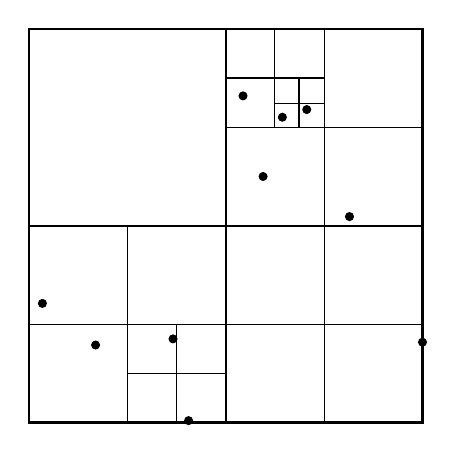
\begin{tikzpicture}[scale=0.05,%
			every circle node/.style = {width=3,fill=black}]
			
% Simulation domain
\draw[thick] (0,0) rectangle (100,100);
\pause
% Level 1
\draw[thick] (50,0) -- (50,100);
\draw[thick] (0,50) -- (100,50);
\draw[fill] (16.9664,19.6802) circle (1); %0
\pause
\draw[fill] (54.4110,82.9573) circle (1); %1
\pause
\draw (0,25) -- (50,25);
\draw (25,0) -- (25,50);
\draw[fill] (03.4614,30.2489) circle (1); %2
\pause
% Level 2
\draw (0,25) -- (100,25);
\draw (75,0) -- (75,100);
\draw (25,0) -- (25,50);
\draw (50,75)-- (100,75);
% Level 3
\draw (25,12.5) -- (50,12.5);
\draw (37.5,0)  -- (37.5,25);
\draw (62.5,75) -- (62.5,100);
\draw (50,87.5) -- (75,87.5);
% Level 4
\draw[thin] (68.625,75) -- (68.625,87.5);
\draw[thin] (62.5,81.125) -- (75,81.125);
% Particles (by increasing id)
\draw[fill] (81.4564,52.3018) circle (1); %3
\draw[fill](59.5102,62.4865) circle (1);  %4
\draw[fill] (40.5800,00.4751) circle (1); %5
\draw[fill] (64.4035,77.5371) circle (1); %6
\draw[fill] (36.6343,21.2396) circle (1); %7
\draw[fill] (99.9970,20.3979) circle (1); %8
\draw[fill] (70.6045,79.4802) circle (1); %9
		\end{tikzpicture}
		\caption{Sample 4-level Barnes-Hut grid with 10 particles.}
		\label{fig:bh-grid}
	\end{figure}
\end{frame}

\begin{frame}
	\frametitle{The Barnes-Hut (Quad-)Tree (Cont.)}
	\begin{figure}
		\centering
		\newlength{\lvld}
		\setlength{\lvld}{7em}
		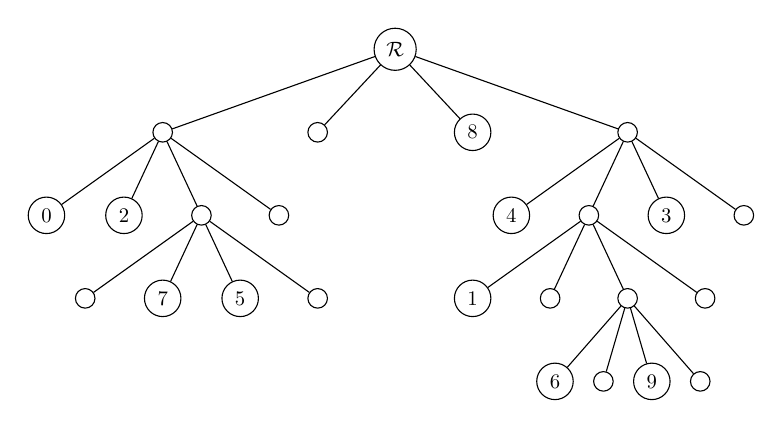
\begin{tikzpicture}[level distance=3em,
		sibling distance=3em,
		level 1/.style={sibling distance=0.80\lvld},
		level 2/.style={sibling distance=0.40\lvld},
		level 3/.style={sibling distance=0.4\lvld},
		level 4/.style={sibling distance=0.25\lvld},
		every node/.style = {shape=circle, draw, align=center, color=black,
			fill=white, scale=0.75}]
		\node {$\mathcal{R}$} %Root
child { node {} %1SW
	child { node{0} } %2SW
	child { node{2} } %2NW
	child { node{} %2SE
		child { node{} } %3SW
		child { node{7} } %3NW
		child { node{5} } %3SE
		child { node{} } } %3NE
	child { node{} } } %2NE
child { node{} }%1NW
child { node{8} }%1SE
child { node{} %1NE
	child { node{4} } %2SW
	child { node{} %2NW
		child { node {1} } %3SW
		child { node {} } %3NW
		child { node {} %3SE
			child { node{6} } %4SW
			child { node{} } %4NW
			child { node{9} } %4SE
			child { node{} } %4SW
		}
		child { node {} } }%3NE
	child { node{3} } %2SE
	child{ node{} } }; %2NE
		\end{tikzpicture}
		\caption{Tree structure associated to the configuration depicted in \cref{fig:bh-grid}.}
	\end{figure}
\end{frame}

\begin{frame}
\frametitle{Parallelization}
The problem is parallelized with MPI.

Each process shall handle a fraction of the simulated particles. We aim for $N\sim10^6\to10^7$.
\end{frame}
